\documentclass[12pt]{article}

\usepackage[T1]{fontenc}
\usepackage{graphicx}
\graphicspath{ {./images/} } 
\usepackage{float}
\begin{document}

(Q)
Describe: ...
\clearpage

SCC361: Artificial Intelligence\\
Week 1: Introduction to Artificial Intelligence and Machine Learning\\
Dr Bryan M. Williams\\
School of Computing and Communications, Lancaster University\\
Office: InfoLab21 C40 Email: b.williams6@lancaster.ac.uk\\
1\\
\begin{figure}[H]

\includegraphics[width=0.5\linewidth]{page1-image-1.png}
\end{figure}
\clearpage
(Q)
Describe: SCC361: Artificial Intelligence
\clearpage
\section{SCC361: Artificial Intelligence}
\\
2\\
Lectures, Materials and Expectations\\
Introduction to the Module\\
Overview of Artificial Intelligence\\
Overview of Machine Learning\\
\begin{figure}[H]

\includegraphics[width=0.5\linewidth]{page2-image-1.png}
\end{figure}
\begin{figure}[H]

\includegraphics[width=0.5\linewidth]{page2-image-2.png}
\end{figure}
\begin{figure}[H]

\includegraphics[width=0.5\linewidth]{page2-image-3.png}
\end{figure}
\begin{figure}[H]

\includegraphics[width=0.5\linewidth]{page2-image-4.png}
\end{figure}
\begin{figure}[H]

\includegraphics[width=0.5\linewidth]{page2-image-5.png}
\end{figure}
\begin{figure}[H]

\includegraphics[width=0.5\linewidth]{page2-image-6.png}
\end{figure}
\begin{figure}[H]

\includegraphics[width=0.5\linewidth]{page2-image-7.png}
\end{figure}
\begin{figure}[H]

\includegraphics[width=0.5\linewidth]{page2-image-8.png}
\end{figure}
\begin{figure}[H]

\includegraphics[width=0.5\linewidth]{page2-image-9.png}
\end{figure}
\begin{figure}[H]

\includegraphics[width=0.5\linewidth]{page2-image-10.png}
\end{figure}
\clearpage
(Q)
Describe: Playing this Video
\clearpage
\section{Playing this Video}
\\
\begin{itemize}
  \item This version is unedited
  \item In general, it might be slow for some people
  \item Vary the playback speed to suit you preferred pace
  \item In live sessions, you can ask questions at any stage, but the 
\end{itemize}
Questions? slides will give you a specific opportunity to ask \\
questions\\
\begin{itemize}
  \item While watching, use the Questions? slides as stop points for 
\end{itemize}
coffee breaks, notes etc\\
3\\
\begin{figure}[H]

\includegraphics[width=0.5\linewidth]{page3-image-1.png}
\end{figure}
\begin{figure}[H]

\includegraphics[width=0.5\linewidth]{page3-image-2.png}
\end{figure}
\begin{figure}[H]

\includegraphics[width=0.5\linewidth]{page3-image-3.png}
\end{figure}
\clearpage
(Q)
Describe: Accessibility
\clearpage
\section{Accessibility}
\\
\begin{itemize}
  \item All our content is expected to meet the UK 
\end{itemize}
accessibility requirements\\
\begin{itemize}
  \item We have done our best to ensure that that is the 
\end{itemize}
case with these course materials\\
\begin{itemize}
  \item However, if any course material or part of its content 
\end{itemize}
is inaccessible in anyway to any individual or group, \\
kindly let us know.\\
4\\
\begin{figure}[H]

\includegraphics[width=0.5\linewidth]{page4-image-1.png}
\end{figure}
\begin{figure}[H]

\includegraphics[width=0.5\linewidth]{page4-image-2.png}
\end{figure}
\begin{figure}[H]
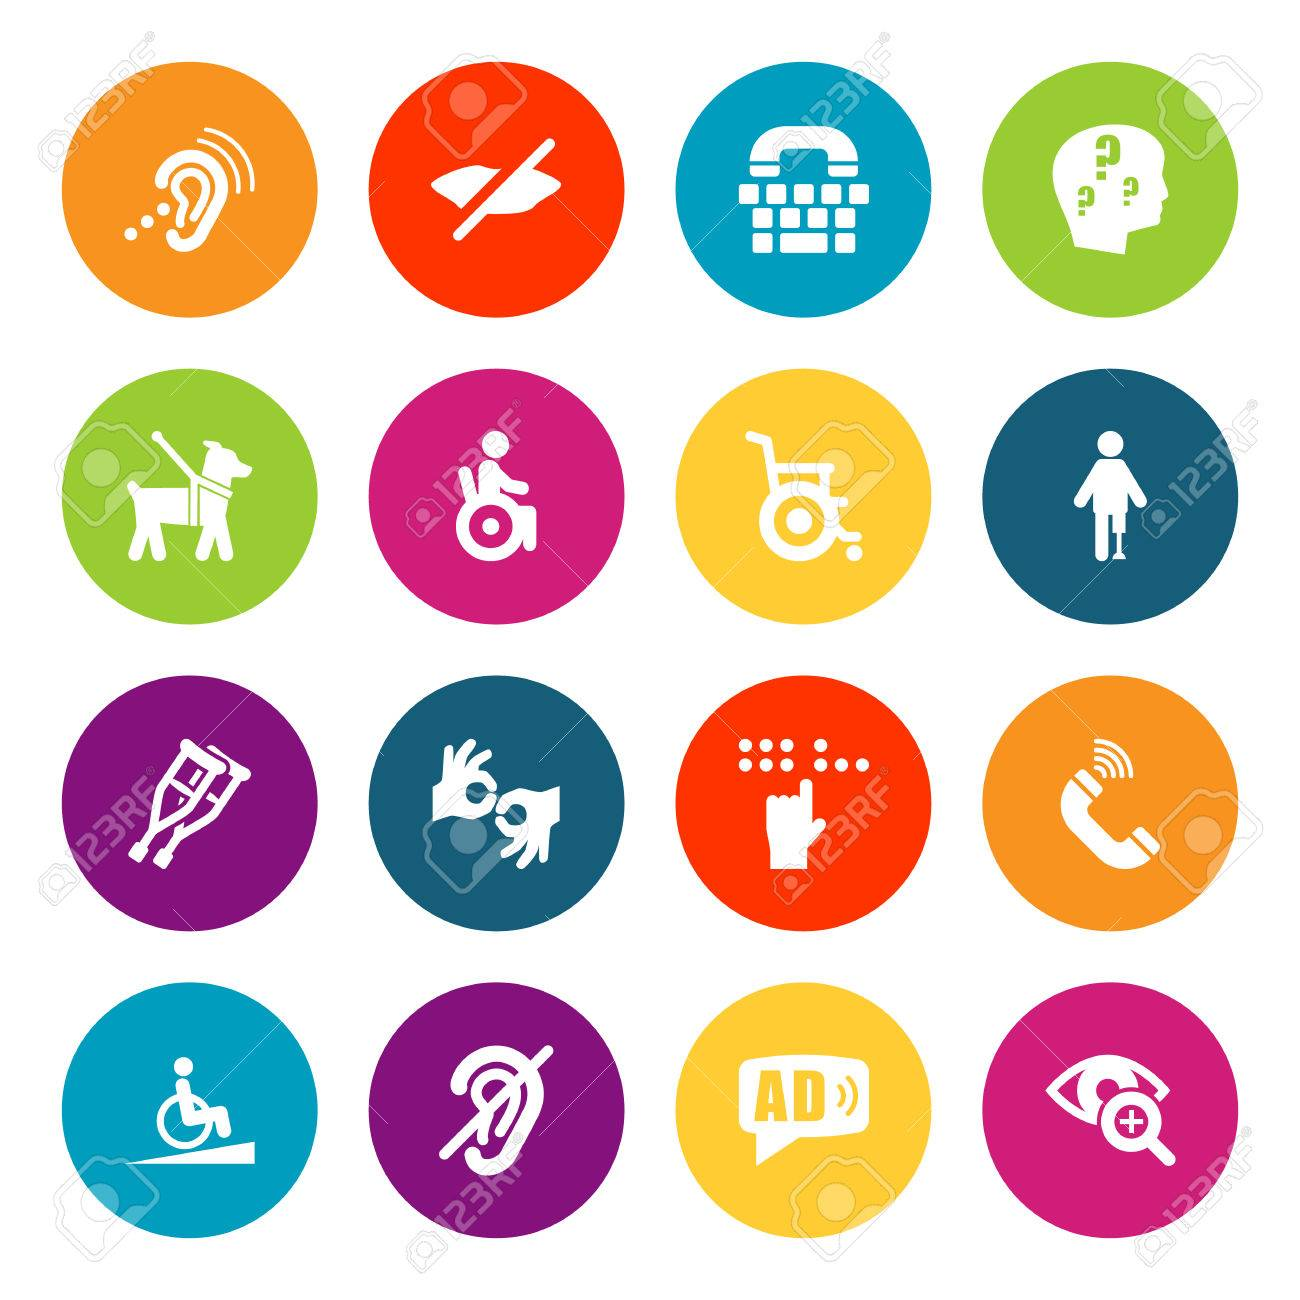
\includegraphics[width=0.5\linewidth]{page4-image-3.png}
\end{figure}
\clearpage
(Q)
Describe: Be sure to check in to all timetabled sessions using 
\clearpage
\section{Be sure to check in to all timetabled sessions using }
\\
Attendance Check-in\\
To check in:\\
\begin{itemize}
  \item Check the Attendance Hub in iLancaster
  \item Click Check In
  \item Wait for the “You are checked in” confirmation page
  \item Here is a the demo
\end{itemize}
Please DO NOT leave a timetabled session without your\\
attendance being registered\\
Attendance Check-in\\
5\\
\begin{figure}[H]

\includegraphics[width=0.5\linewidth]{page5-image-1.png}
\end{figure}
\begin{figure}[H]

\includegraphics[width=0.5\linewidth]{page5-image-2.png}
\end{figure}
\begin{figure}[H]

\includegraphics[width=0.5\linewidth]{page5-image-3.png}
\end{figure}
\clearpage
(Q)
Describe: Online Sessions on Teams
\clearpage
\section{Online Sessions on Teams}
\\
Before the session:\\
\begin{itemize}
  \item Follow the Moodle link to join the lecture
  \item Ensure that your speakers, headsets are connected and working
\end{itemize}
6\\
\begin{figure}[H]

\includegraphics[width=0.5\linewidth]{page6-image-1.png}
\end{figure}
\begin{figure}[H]

\includegraphics[width=0.5\linewidth]{page6-image-2.png}
\end{figure}
\begin{figure}[H]

\includegraphics[width=0.5\linewidth]{page6-image-3.png}
\end{figure}
\clearpage
(Q)
Describe: Online Sessions on Teams
\clearpage
\section{Online Sessions on Teams}
\\
During the lectures:\\
\begin{itemize}
  \item Turn your webcam off
  \item Turn your microphone off
\end{itemize}
7\\
\begin{figure}[H]

\includegraphics[width=0.5\linewidth]{page7-image-1.png}
\end{figure}
\begin{figure}[H]

\includegraphics[width=0.5\linewidth]{page7-image-2.png}
\end{figure}
\begin{figure}[H]

\includegraphics[width=0.5\linewidth]{page7-image-3.png}
\end{figure}
\clearpage
(Q)
Describe: Online Sessions on Teams
\clearpage
\section{Online Sessions on Teams}
\\
During the lectures:\\
\begin{itemize}
  \item Use  chat  appropriately. Not closely monitored during lectures.
\end{itemize}
For live Q\&A sessions:\\
\begin{itemize}
  \item Raise your hand to ask questions. Lower it afterwards.
  \item When called, turn on your mic (and cam if you wish). Remember to turn them off 
\end{itemize}
afterwards.\\
Post additional questions on the SCC361 Moodle Forum\\
8\\
\begin{figure}[H]

\includegraphics[width=0.5\linewidth]{page8-image-1.png}
\end{figure}
\begin{figure}[H]

\includegraphics[width=0.5\linewidth]{page8-image-2.png}
\end{figure}
\begin{figure}[H]

\includegraphics[width=0.5\linewidth]{page8-image-3.png}
\end{figure}
\clearpage
(Q)
Describe: Online Sessions on Teams
\clearpage
\section{Online Sessions on Teams}
\\
After the lectures:\\
\begin{itemize}
  \item The recorded content of the live sessions will be made available after the session on the 
\end{itemize}
Moodle Space\\
9\\
\begin{figure}[H]

\includegraphics[width=0.5\linewidth]{page9-image-1.png}
\end{figure}
\begin{figure}[H]

\includegraphics[width=0.5\linewidth]{page9-image-2.png}
\end{figure}
\begin{figure}[H]

\includegraphics[width=0.5\linewidth]{page9-image-3.png}
\end{figure}
\clearpage
(Q)
Describe: The lectures can be watched on the Moodle space.
\clearpage
\section{The lectures can be watched on the Moodle space.}
\\
If you are struggling to watch the videos on Moodle:\\
\begin{itemize}
  \item Download the video and caption file (*.vtt) from Moodle
  \item Download the free, open source VLC Media player: 
\end{itemize}
https://www.videolan.org/vlc/index.en-GB.html\\
\begin{itemize}
  \item Open video file in VLC and add caption file
\end{itemize}
Note:\\
All learning materials: slides, videos and caption\\
files are @Lancaster University copyright and are \\
not to be shared or distributed.\\
Using Materials Offline\\
10\\
\begin{figure}[H]

\includegraphics[width=0.5\linewidth]{page10-image-1.png}
\end{figure}
\begin{figure}[H]

\includegraphics[width=0.5\linewidth]{page10-image-2.png}
\end{figure}
\begin{figure}[H]
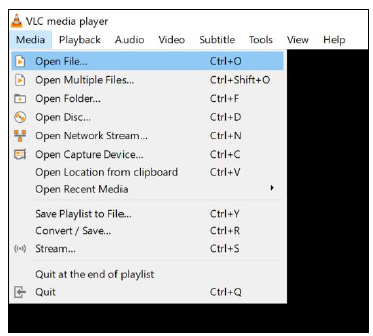
\includegraphics[width=0.5\linewidth]{page10-image-3.png}
\end{figure}
\begin{figure}[H]
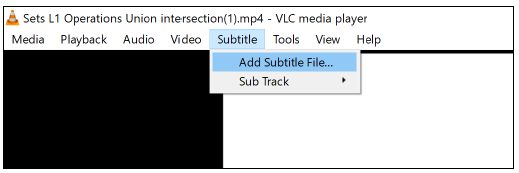
\includegraphics[width=0.5\linewidth]{page10-image-4.png}
\end{figure}
\clearpage
(Q)
Describe: Passing off someone else’s work as your own, including:
\clearpage
\section{Passing off someone else’s work as your own, including:}
\\
\begin{itemize}
  \item Colluding with a classmate or someone else to do your work
  \item Submitting code written by someone else
  \item Paying for someone else to do your work
  \item Adapting code by someone else with only a minor modification
  \item Course work is submitted on Moodle and will be checked automatically for plagiarism!
\end{itemize}
Plagiarism\\
11\\
\begin{itemize}
  \item \begin{figure}[H]

\includegraphics[width=0.5\linewidth]{page11-image-1.png}
\end{figure}
\begin{figure}[H]

\includegraphics[width=0.5\linewidth]{page11-image-2.png}
\end{figure}
\clearpage
(Q)
Describe: Online tools will be used to facilitate some aspects of learning e.g. Moodle, Teams, etc.
\clearpage
\section{Online tools will be used to facilitate some aspects of learning e.g. Moodle, Teams, etc.}

  \item The use of these is governed by existing policies that you are all currently bound by and 
\end{itemize}
have agreed to\\
\begin{itemize}
  \item Academic malpractice and plagiarism still applies online
  \item Direct sharing of code, sharing solutions and/or partial solutions with other students, 
\end{itemize}
either privately or in an open chat, is not acceptable\\
Online Learning Expectations\\
12\\
\begin{itemize}
  \item \begin{figure}[H]

\includegraphics[width=0.5\linewidth]{page12-image-1.png}
\end{figure}
\begin{figure}[H]

\includegraphics[width=0.5\linewidth]{page12-image-2.png}
\end{figure}
\clearpage
(Q)
Describe: Don’t forget, these are your fellow students and staff, not some anonymous person on 
\clearpage
\section{Don’t forget, these are your fellow students and staff, not some anonymous person on }

\end{itemize}
the Internet\\
\begin{itemize}
  \item If you’re not sure if you should post or share something, please ask first
  \item If you see content or a post that you don’t like, in the first instance, message or email 
\end{itemize}
the course tutor to alert them to it\\
\begin{itemize}
  \item We want these tools to be used; they will give you the best online experience!
  \item However, we are asking that you use them sensibly and with respect
\end{itemize}
Online Learning Expectations\\
13\\
\begin{figure}[H]

\includegraphics[width=0.5\linewidth]{page13-image-1.png}
\end{figure}
\begin{figure}[H]

\includegraphics[width=0.5\linewidth]{page13-image-2.png}
\end{figure}
\clearpage
(Q)
Describe: Attendance:
\clearpage
\section{Attendance:}
\\
\begin{itemize}
  \item Lectures, labs etc., be punctual
\end{itemize}
Active learning:\\
\begin{itemize}
  \item Read around (explore) the subject
  \item Use recommended books and available online resources
  \item Ask questions, try things yourself, keep notes
  \item Have a study plan, get a study partner
\end{itemize}
Integrity:\\
\begin{itemize}
  \item Honesty, no plagiarism/ result manipulation
\end{itemize}
What do we expect from you?\\
14\\
\begin{itemize}
  \item \begin{figure}[H]

\includegraphics[width=0.5\linewidth]{page14-image-1.png}
\end{figure}
\begin{figure}[H]

\includegraphics[width=0.5\linewidth]{page14-image-2.png}
\end{figure}
\clearpage
(Q)
Describe: Lecture slides and videos will be available on Moodle
\clearpage
\section{Lecture slides and videos will be available on Moodle}

  \item Provide references to follow up
  \item TAs will be available to ensure that the labs are running smoothly
  \item Arrange extra support if you are struggling and let us know on time
  \item Provide prompt feedback on formative coursework
  \item In extreme cases, respond to coursework questions outside the labs
  \item We encourage you to maximise the use of lab sessions for all coursework related 
\end{itemize}
questions\\
How can we help?\\
15\\
\begin{itemize}
  \item \begin{figure}[H]

\includegraphics[width=0.5\linewidth]{page15-image-1.png}
\end{figure}
\begin{figure}[H]

\includegraphics[width=0.5\linewidth]{page15-image-2.png}
\end{figure}
\clearpage
(Q)
Describe: Use the labs to ask TAs/Tutors for help
\clearpage
\section{Use the labs to ask TAs/Tutors for help}

  \item Use the course forum on Moodle
  \item Check other available (online) resources
  \item Drop me an email/ ask on Teams chat
  \item There might be delays in replying
\end{itemize}
How to get help\\
16\\
\begin{figure}[H]

\includegraphics[width=0.5\linewidth]{page16-image-1.png}
\end{figure}
\begin{figure}[H]

\includegraphics[width=0.5\linewidth]{page16-image-2.png}
\end{figure}
\clearpage
(Q)
Describe: Questions?
\clearpage
\section{Questions?}
\\
17\\
\begin{figure}[H]

\includegraphics[width=0.5\linewidth]{page17-image-1.png}
\end{figure}
\begin{figure}[H]

\includegraphics[width=0.5\linewidth]{page17-image-2.png}
\end{figure}
\begin{figure}[H]
\includegraphics[width=0.5\linewidth]{page17-image-3.png}
\end{figure}
\clearpage
(Q)
Describe: SCC361: Artificial Intelligence
\clearpage
\section{SCC361: Artificial Intelligence}
\\
18\\
Lectures, Materials and Expectations\\
Introduction to the Module\\
Overview of Artificial Intelligence\\
Overview of Machine Learning\\
\begin{figure}[H]
\includegraphics[width=0.5\linewidth]{page18-image-1.png}
\end{figure}
\begin{figure}[H]
\includegraphics[width=0.5\linewidth]{page18-image-2.png}
\end{figure}
\begin{figure}[H]
\includegraphics[width=0.5\linewidth]{page18-image-3.png}
\end{figure}
\begin{figure}[H]
\includegraphics[width=0.5\linewidth]{page18-image-4.png}
\end{figure}
\begin{figure}[H]
\includegraphics[width=0.5\linewidth]{page18-image-5.png}
\end{figure}
\begin{figure}[H]
\includegraphics[width=0.5\linewidth]{page18-image-6.png}
\end{figure}
\begin{figure}[H]
\includegraphics[width=0.5\linewidth]{page18-image-7.png}
\end{figure}
\begin{figure}[H]
\includegraphics[width=0.5\linewidth]{page18-image-8.png}
\end{figure}
\begin{figure}[H]
\includegraphics[width=0.5\linewidth]{page18-image-9.png}
\end{figure}
\begin{figure}[H]
\includegraphics[width=0.5\linewidth]{page18-image-10.png}
\end{figure}
\clearpage
(Q)
Describe: In this video
\clearpage
\section{In this video}
\\
\begin{itemize}
  \item Expected Learning Outcomes
  \item Teaching Staff
  \item Lecture Plan
  \item Teaching Structure
  \item Assessment
\end{itemize}
19\\
\begin{figure}[H]
\includegraphics[width=0.5\linewidth]{page19-image-1.png}
\end{figure}
\begin{figure}[H]
\includegraphics[width=0.5\linewidth]{page19-image-2.png}
\end{figure}
\begin{figure}[H]
\includegraphics[width=0.5\linewidth]{page19-image-3.png}
\end{figure}
\clearpage
(Q)
Describe: Expected Learning Outcomes
\clearpage
\section{Expected Learning Outcomes}
\\
We will to be able to:\\
\begin{itemize}
  \item understand AI concepts, applications and trends
  \item understand machine learning terms
  \item train machine learning models for specific tasks
  \item learn implement simple AI-based systems
  \item learn how to evaluate the performance of AI systems
\end{itemize}
20\\
\begin{figure}[H]
\includegraphics[width=0.5\linewidth]{page20-image-1.png}
\end{figure}
\begin{figure}[H]
\includegraphics[width=0.5\linewidth]{page20-image-2.png}
\end{figure}
\begin{figure}[H]
\includegraphics[width=0.5\linewidth]{page20-image-3.png}
\end{figure}
\begin{figure}[H]
\includegraphics[width=0.5\linewidth]{page20-image-4.png}
\end{figure}
\clearpage
(Q)
Describe: Teaching Staff
\clearpage
\section{Teaching Staff}
\\
21\\
Dr Bryan M. Williams\\
Weeks 1-5\\
Dr Hossein Rahmani\\
Weeks 6-10\\
Module Convenor\\
Teaching Assistants Group 1 Group 2 Group 3 Group 4 Group 5\\
Mona Alghamdi\\
Somayeh Bazin\\
Piotr Daniszewski\\
Oishi Deb\\
Ovini Gunasekera\\
Yuri Tavares dos Passos\\
\begin{figure}[H]
\includegraphics[width=0.5\linewidth]{page21-image-1.png}
\end{figure}
\begin{figure}[H]
\includegraphics[width=0.5\linewidth]{page21-image-2.png}
\end{figure}
\begin{figure}[H]
\includegraphics[width=0.5\linewidth]{page21-image-3.png}
\end{figure}
\begin{figure}[H]
\includegraphics[width=0.5\linewidth]{page21-image-4.png}
\end{figure}
\clearpage
(Q)
Describe: Lecture Plan
\clearpage
\section{Lecture Plan}
\\
Weeks 1-5\\
1. Introduction to Artificial Intelligence \\
and Machine Learning\\
2. Features in Machine Learning and \\
Feature Extraction\\
3. Computer Vision and Natura Language \\
Processing\\
4. Clustering and Classification\\
5. Artificial Neural Networks\\
Weeks 6-10:\\
6. Genetic Algorithms\\
7. Naïve Bayesian Classifier\\
8. Decision Tree Classifier\\
9. Introduction to Deep Neural Networks\\
10. Introduction to Convolutional Neural \\
Networks\\
22\\
\begin{figure}[H]
\includegraphics[width=0.5\linewidth]{page22-image-1.png}
\end{figure}
\begin{figure}[H]
\includegraphics[width=0.5\linewidth]{page22-image-2.png}
\end{figure}
\clearpage
(Q)
Describe: Teaching Structure
\clearpage
\section{Teaching Structure}
\\
Lectures:\\
\begin{itemize}
  \item Weeks 1-10
  \item Online only
  \item Mondays: 14.00-15.00
  \item Tuesdays: 17.00-18.00
\end{itemize}
Labs:\\
\begin{itemize}
  \item Weeks 1-10
  \item Blended: in-person and online
  \item Wednesdays: 11.00-13.00
  \item Thursdays: 10.00-12.00
  \item Thursdays: 16.00-18.00
  \item Fridays: 11.00-13.00
  \item Fridays: 16.00-18.00
\end{itemize}
23\\
\begin{figure}[H]
\includegraphics[width=0.5\linewidth]{page23-image-1.png}
\end{figure}
\begin{figure}[H]
\includegraphics[width=0.5\linewidth]{page23-image-2.png}
\end{figure}
\clearpage
(Q)
Describe: Teaching Structure
\clearpage
\section{Teaching Structure}
\\
Labs:\\
24\\
Group Day Time Room\\
SCC361/P01/01 Wednesday 11:00-13:00 FST B076\\
SCC361/P01/02 Thursday 16:00-18:00 FST B076\\
SCC361/P01/03 Friday 16:00-18:00 (Weeks 1-4, 6, 8, 10)\\
14:00-16:00 (Weeks 5, 7, 9)\\
FST B070 (Weeks 1-4)\\
FST B074 (Weeks 5, 7, 9)\\
FST B080 (Weeks 6, 8, 10)\\
SCC361/P01/04 Thursday 10:00-12:00 FST B070\\
SCC361/P01/05 Friday 11:00-13:00 FST B080\\
\begin{figure}[H]
\includegraphics[width=0.5\linewidth]{page24-image-1.png}
\end{figure}
\begin{figure}[H]
\includegraphics[width=0.5\linewidth]{page24-image-2.png}
\end{figure}
\clearpage
(Q)
Describe: 2 Courseworks: 40\%
\clearpage
\section{2 Courseworks: 40\%}
\\
\begin{itemize}
  \item CW1 (20marks):
  \item Submission: On Moodle
  \item Deadline: 5pm Friday 12th November, 2021
  \item CW2 (20marks):
  \item Details: to be confirmed
\end{itemize}
Exam: 60\%\\
\begin{itemize}
  \item Next semester in 2021
  \item Date: To be confirmed
\end{itemize}
Assessment\\
25\\
\begin{figure}[H]
\includegraphics[width=0.5\linewidth]{page25-image-1.png}
\end{figure}
\begin{figure}[H]
\includegraphics[width=0.5\linewidth]{page25-image-2.png}
\end{figure}
\clearpage
(Q)
Describe: Questions?
\clearpage
\section{Questions?}
\\
26\\
\begin{figure}[H]
\includegraphics[width=0.5\linewidth]{page26-image-1.png}
\end{figure}
\begin{figure}[H]
\includegraphics[width=0.5\linewidth]{page26-image-2.png}
\end{figure}
\begin{figure}[H]
\includegraphics[width=0.5\linewidth]{page26-image-3.png}
\end{figure}
\clearpage
(Q)
Describe: SCC361: Artificial Intelligence
\clearpage
\section{SCC361: Artificial Intelligence}
\\
27\\
Lectures, Materials and Expectations\\
Introduction to the Module\\
Overview of Artificial Intelligence\\
Overview of Machine Learning\\
\begin{figure}[H]
\includegraphics[width=0.5\linewidth]{page27-image-1.png}
\end{figure}
\begin{figure}[H]
\includegraphics[width=0.5\linewidth]{page27-image-2.png}
\end{figure}
\begin{figure}[H]
\includegraphics[width=0.5\linewidth]{page27-image-3.png}
\end{figure}
\begin{figure}[H]
\includegraphics[width=0.5\linewidth]{page27-image-4.png}
\end{figure}
\begin{figure}[H]
\includegraphics[width=0.5\linewidth]{page27-image-5.png}
\end{figure}
\begin{figure}[H]
\includegraphics[width=0.5\linewidth]{page27-image-6.png}
\end{figure}
\begin{figure}[H]
\includegraphics[width=0.5\linewidth]{page27-image-7.png}
\end{figure}
\begin{figure}[H]
\includegraphics[width=0.5\linewidth]{page27-image-8.png}
\end{figure}
\begin{figure}[H]
\includegraphics[width=0.5\linewidth]{page27-image-9.png}
\end{figure}
\begin{figure}[H]
\includegraphics[width=0.5\linewidth]{page27-image-10.png}
\end{figure}
\clearpage
(Q)
Describe: Part 1 (Weeks 1 – 5):
\clearpage
\section{Part 1 (Weeks 1 – 5):}
\\
\begin{itemize}
  \item Wk1: Intro to Artificial Intelligence \& Machine Learning
  \item Wk2: What are features and how to extract features from texts, 
\end{itemize}
images, etc.\\
\begin{itemize}
  \item Wk3: Computer Vision and Natural Language Processing
  \item Wk4: Clustering \& Classification
  \item Wk5: Intro to Artificial Neural Networks \& Review of Previous 
\end{itemize}
Lectures\\
Part 2 (Weeks 6 – 10):\\
\begin{itemize}
  \item Dr Hossein Rahmani (GAs, NBCs, DTCs, DNNs, CNNs)
\end{itemize}
Welcome to SCC361\\
28\\
\begin{figure}[H]
\includegraphics[width=0.5\linewidth]{page28-image-1.png}
\end{figure}
\begin{figure}[H]
\includegraphics[width=0.5\linewidth]{page28-image-2.png}
\end{figure}
\begin{figure}[H]
\includegraphics[width=0.5\linewidth]{page28-image-3.png}
\end{figure}
\clearpage
(Q)
Describe: Artificial Intelligence: An Overview
\clearpage
\section{Artificial Intelligence: An Overview}
\\
\begin{itemize}
  \item Application, history, foundations of AI
  \item Definition of AI
  \item Goals of AI
  \item AI and the Society
  \item Benefits
  \item Risk and Challenges
  \item Ethical Issues
\end{itemize}
This Week’s Lectures\\
29\\
\begin{figure}[H]
\includegraphics[width=0.5\linewidth]{page29-image-1.png}
\end{figure}
\begin{figure}[H]
\includegraphics[width=0.5\linewidth]{page29-image-2.png}
\end{figure}
\begin{figure}[H]
\includegraphics[width=0.5\linewidth]{page29-image-3.png}
\end{figure}
\clearpage
(Q)
Describe: Overview of Machine Learning
\clearpage
\section{Overview of Machine Learning}
\\
\begin{itemize}
  \item AI and ML, Definitions of ML, How to learn
\end{itemize}
Types of Machine Learning\\
\begin{itemize}
  \item Supervised, unsupervised, semi supervised
\end{itemize}
Supervised Learning\\
\begin{itemize}
  \item Classification and regression
\end{itemize}
Unsupervised Learning\\
\begin{itemize}
  \item Clustering and association
\end{itemize}
This Week’s Lectures\\
30\\
\begin{itemize}
  \item \begin{figure}[H]
\includegraphics[width=0.5\linewidth]{page30-image-1.png}
\end{figure}
\begin{figure}[H]
\includegraphics[width=0.5\linewidth]{page30-image-2.png}
\end{figure}
\begin{figure}[H]
\includegraphics[width=0.5\linewidth]{page30-image-3.png}
\end{figure}
\clearpage
(Q)
Describe: Artificial Intelligence: Foundations of Computational 
\clearpage
\section{Artificial Intelligence: Foundations of Computational }

\end{itemize}
Agents 2ed. Poole \& Mackworth 2017\\
\begin{itemize}
  \item Artificial Intelligence A Modern Approach, Russell \& 
\end{itemize}
Norvig, 2016 (chapters 1,2,5,6)\\
\begin{itemize}
  \item Deep Learning, Goodfellow et al. , 2016
  \item Deep Learning with PyTorch, Stevens et al, 2020.
  \item Machine Learning, T. M. Mitchell, 1997
  \item Artificial Intelligence on Wikipedia
  \item Many online resources
\end{itemize}
Recommended Reading\\
31\\
\begin{figure}[H]
\includegraphics[width=0.5\linewidth]{page31-image-1.png}
\end{figure}
\begin{figure}[H]
\includegraphics[width=0.5\linewidth]{page31-image-2.png}
\end{figure}
\begin{figure}[H]
\includegraphics[width=0.5\linewidth]{page31-image-3.png}
\end{figure}
\clearpage
(Q)
Describe: SCC361: Week 1
\clearpage
\section{SCC361: Week 1}
\\
32\\
\begin{itemize}
  \item AI Overview
  \item Definition of AI
  \item Goals of AI
  \item AI and Society
\end{itemize}
Artificial Intelligence\\
\begin{itemize}
  \item Machine Learning Overview
  \item Types of Machine Learning
  \item Supervised Learning
  \item Unsupervised Learning
\end{itemize}
Introduction to Machine Learning\\
\begin{figure}[H]
\includegraphics[width=0.5\linewidth]{page32-image-1.png}
\end{figure}
\begin{figure}[H]
\includegraphics[width=0.5\linewidth]{page32-image-2.png}
\end{figure}
\clearpage
(Q)
Describe: AI in Real Life
\clearpage
\section{AI in Real Life}
\\
33\\
\begin{figure}[H]
\includegraphics[width=0.5\linewidth]{page33-image-1.png}
\end{figure}
\begin{figure}[H]
\includegraphics[width=0.5\linewidth]{page33-image-2.png}
\end{figure}
\begin{figure}[H]
\includegraphics[width=0.5\linewidth]{page33-image-3.png}
\end{figure}
\begin{figure}[H]
\includegraphics[width=0.5\linewidth]{page33-image-4.png}
\end{figure}
\begin{figure}[H]
\includegraphics[width=0.5\linewidth]{page33-image-5.png}
\end{figure}
\begin{figure}[H]
\includegraphics[width=0.5\linewidth]{page33-image-6.png}
\end{figure}
\begin{figure}[H]
\includegraphics[width=0.5\linewidth]{page33-image-7.png}
\end{figure}
\begin{figure}[H]
\includegraphics[width=0.5\linewidth]{page33-image-8.png}
\end{figure}
\clearpage
(Q)
Describe: AI in Science Fiction Movies
\clearpage
\section{AI in Science Fiction Movies}
\\
34\\
\begin{figure}[H]
\includegraphics[width=0.5\linewidth]{page34-image-1.png}
\end{figure}
\begin{figure}[H]
\includegraphics[width=0.5\linewidth]{page34-image-2.png}
\end{figure}
\begin{figure}[H]
\includegraphics[width=0.5\linewidth]{page34-image-3.png}
\end{figure}
\begin{figure}[H]
\includegraphics[width=0.5\linewidth]{page34-image-4.png}
\end{figure}
\begin{figure}[H]
\includegraphics[width=0.5\linewidth]{page34-image-5.png}
\end{figure}
\begin{figure}[H]
\includegraphics[width=0.5\linewidth]{page34-image-6.png}
\end{figure}
\begin{figure}[H]
\includegraphics[width=0.5\linewidth]{page34-image-7.png}
\end{figure}
\clearpage
(Q)
Describe: AI in Science Fiction Movies
\clearpage
\section{AI in Science Fiction Movies}
\\
35\\
\begin{figure}[H]
\includegraphics[width=0.5\linewidth]{page35-image-1.png}
\end{figure}
\begin{figure}[H]
\includegraphics[width=0.5\linewidth]{page35-image-2.png}
\end{figure}
\begin{figure}[H]
\includegraphics[width=0.5\linewidth]{page35-image-3.png}
\end{figure}
\begin{figure}[H]
\includegraphics[width=0.5\linewidth]{page35-image-4.png}
\end{figure}
\begin{figure}[H]
\includegraphics[width=0.5\linewidth]{page35-image-5.png}
\end{figure}
\clearpage
(Q)
Describe: AI in Music
\clearpage
\section{AI in Music}
\\
36\\
\begin{figure}[H]
\includegraphics[width=0.5\linewidth]{page36-image-1.png}
\end{figure}
\begin{figure}[H]
\includegraphics[width=0.5\linewidth]{page36-image-2.png}
\end{figure}
\begin{figure}[H]
\includegraphics[width=0.5\linewidth]{page36-image-3.png}
\end{figure}
\begin{figure}[H]
\includegraphics[width=0.5\linewidth]{page36-image-4.png}
\end{figure}
\clearpage
(Q)
Describe: AI in Agriculture
\clearpage
\section{AI in Agriculture}
\\
37\\
\begin{figure}[H]
\includegraphics[width=0.5\linewidth]{page37-image-1.png}
\end{figure}
\begin{figure}[H]
\includegraphics[width=0.5\linewidth]{page37-image-2.png}
\end{figure}
\begin{figure}[H]
\includegraphics[width=0.5\linewidth]{page37-image-3.png}
\end{figure}
\begin{figure}[H]
\includegraphics[width=0.5\linewidth]{page37-image-4.png}
\end{figure}
\clearpage
(Q)
Describe: AI in Delivery Services
\clearpage
\section{AI in Delivery Services}
\\
38\\
\begin{figure}[H]
\includegraphics[width=0.5\linewidth]{page38-image-1.png}
\end{figure}
\begin{figure}[H]
\includegraphics[width=0.5\linewidth]{page38-image-2.png}
\end{figure}
\begin{figure}[H]
\includegraphics[width=0.5\linewidth]{page38-image-3.png}
\end{figure}
\begin{figure}[H]
\includegraphics[width=0.5\linewidth]{page38-image-4.png}
\end{figure}
\begin{figure}[H]
\includegraphics[width=0.5\linewidth]{page38-image-5.png}
\end{figure}
\clearpage
(Q)
Describe: AI in Self-Driving Vehicles
\clearpage
\section{AI in Self-Driving Vehicles}
\\
39\\
\begin{figure}[H]
\includegraphics[width=0.5\linewidth]{page39-image-1.png}
\end{figure}
\begin{figure}[H]
\includegraphics[width=0.5\linewidth]{page39-image-2.png}
\end{figure}
\begin{figure}[H]
\includegraphics[width=0.5\linewidth]{page39-image-3.png}
\end{figure}
\begin{figure}[H]
\includegraphics[width=0.5\linewidth]{page39-image-4.png}
\end{figure}
\clearpage
(Q)
Describe: AI in Medicine
\clearpage
\section{AI in Medicine}
\\
40\\
\begin{figure}[H]
\includegraphics[width=0.5\linewidth]{page40-image-1.png}
\end{figure}
\begin{figure}[H]
\includegraphics[width=0.5\linewidth]{page40-image-2.png}
\end{figure}
\begin{figure}[H]
\includegraphics[width=0.5\linewidth]{page40-image-3.png}
\end{figure}
\clearpage
(Q)
Describe: AI in Medicine
\clearpage
\section{AI in Medicine}
\\
41\\
\begin{figure}[H]
\includegraphics[width=0.5\linewidth]{page41-image-1.png}
\end{figure}
\begin{figure}[H]
\includegraphics[width=0.5\linewidth]{page41-image-2.png}
\end{figure}
\begin{figure}[H]
\includegraphics[width=0.5\linewidth]{page41-image-3.png}
\end{figure}
\clearpage
(Q)
Describe: AI in Medicine
\clearpage
\section{AI in Medicine}
\\
42\\
\begin{figure}[H]
\includegraphics[width=0.5\linewidth]{page42-image-1.png}
\end{figure}
\begin{figure}[H]
\includegraphics[width=0.5\linewidth]{page42-image-2.png}
\end{figure}
\begin{figure}[H]
\includegraphics[width=0.5\linewidth]{page42-image-3.png}
\end{figure}
\begin{figure}[H]
\includegraphics[width=0.5\linewidth]{page42-image-4.png}
\end{figure}
\begin{figure}[H]
\includegraphics[width=0.5\linewidth]{page42-image-5.png}
\end{figure}
\begin{figure}[H]
\includegraphics[width=0.5\linewidth]{page42-image-6.png}
\end{figure}
\begin{figure}[H]
\includegraphics[width=0.5\linewidth]{page42-image-7.png}
\end{figure}
\clearpage
(Q)
Describe: AI in Medicine
\clearpage
\section{AI in Medicine}
\\
43\\
\begin{figure}[H]
\includegraphics[width=0.5\linewidth]{page43-image-1.png}
\end{figure}
\begin{figure}[H]
\includegraphics[width=0.5\linewidth]{page43-image-2.png}
\end{figure}
\begin{figure}[H]
\includegraphics[width=0.5\linewidth]{page43-image-3.png}
\end{figure}
\begin{figure}[H]
\includegraphics[width=0.5\linewidth]{page43-image-4.png}
\end{figure}
\begin{figure}[H]
\includegraphics[width=0.5\linewidth]{page43-image-5.png}
\end{figure}
\clearpage
(Q)
Describe: AI in Security
\clearpage
\section{AI in Security}
\\
44\\
\begin{figure}[H]
\includegraphics[width=0.5\linewidth]{page44-image-1.png}
\end{figure}
\begin{figure}[H]
\includegraphics[width=0.5\linewidth]{page44-image-2.png}
\end{figure}
\begin{figure}[H]
\includegraphics[width=0.5\linewidth]{page44-image-3.png}
\end{figure}
\begin{figure}[H]
\includegraphics[width=0.5\linewidth]{page44-image-4.png}
\end{figure}
\begin{figure}[H]
\includegraphics[width=0.5\linewidth]{page44-image-5.png}
\end{figure}
\clearpage
(Q)
Describe: AI in Forensic Identification
\clearpage
\section{AI in Forensic Identification}
\\
45\\
https://h-unique.lancaster.ac.uk/\\
\begin{itemize}
  \item \begin{figure}[H]
\includegraphics[width=0.5\linewidth]{page45-image-1.png}
\end{figure}
\begin{figure}[H]
\includegraphics[width=0.5\linewidth]{page45-image-2.png}
\end{figure}
\begin{figure}[H]
\includegraphics[width=0.5\linewidth]{page45-image-3.png}
\end{figure}
\begin{figure}[H]
\includegraphics[width=0.5\linewidth]{page45-image-4.png}
\end{figure}
\begin{figure}[H]
\includegraphics[width=0.5\linewidth]{page45-image-5.png}
\end{figure}
\begin{figure}[H]
\includegraphics[width=0.5\linewidth]{page45-image-6.png}
\end{figure}
\begin{figure}[H]
\includegraphics[width=0.5\linewidth]{page45-image-7.png}
\end{figure}
\clearpage
(Q)
Describe: Web search engines
\clearpage
\section{Web search engines}

  \item Text classification: sentiment, topic
  \item Spam filtering etc
  \item Machine translation
  \item Question answering
  \item Recommender Systems
\end{itemize}
AI in Natural Language Processing\\
46\\
\begin{figure}[H]
\includegraphics[width=0.5\linewidth]{page46-image-1.png}
\end{figure}
\begin{figure}[H]
\includegraphics[width=0.5\linewidth]{page46-image-2.png}
\end{figure}
\begin{figure}[H]
\includegraphics[width=0.5\linewidth]{page46-image-3.png}
\end{figure}
\begin{figure}[H]
\includegraphics[width=0.5\linewidth]{page46-image-4.png}
\end{figure}
\begin{figure}[H]
\includegraphics[width=0.5\linewidth]{page46-image-5.png}
\end{figure}
\begin{figure}[H]
\includegraphics[width=0.5\linewidth]{page46-image-6.png}
\end{figure}
\begin{figure}[H]
\includegraphics[width=0.5\linewidth]{page46-image-7.png}
\end{figure}
\clearpage
(Q)
Describe: Speech Technologies
\clearpage
\section{Speech Technologies}
\\
\begin{itemize}
  \item Siri, Alexa, Cortana, Google Assistant
  \item Automatic Speech Recognition
  \item Dialogue systems
\end{itemize}
AI in Natural Language Processing\\
47\\
\begin{figure}[H]
\includegraphics[width=0.5\linewidth]{page47-image-1.png}
\end{figure}
\begin{figure}[H]
\includegraphics[width=0.5\linewidth]{page47-image-2.png}
\end{figure}
\begin{figure}[H]
\includegraphics[width=0.5\linewidth]{page47-image-3.png}
\end{figure}
\begin{figure}[H]
\includegraphics[width=0.5\linewidth]{page47-image-4.png}
\end{figure}
\begin{figure}[H]
\includegraphics[width=0.5\linewidth]{page47-image-5.png}
\end{figure}
\begin{figure}[H]
\includegraphics[width=0.5\linewidth]{page47-image-6.png}
\end{figure}
\clearpage
(Q)
Describe: Brief History of AI
\clearpage
\section{Brief History of AI}
\\
48\\
1940-1950: Early Days\\
\begin{itemize}
  \item 1943: McCulloch \& Pitts: 
\end{itemize}
Boolean Circuit Model of \\
Brain\\
\begin{itemize}
  \item 1950: Turing's “Computing 
\end{itemize}
Machinery and \\
Intelligence”\\
1950-1970: Excitement\\
\begin{itemize}
  \item 1950s: Early AI programs: 
\end{itemize}
Samuel's checkers \\
program, Newell \& \\
Simon's Logic Theorist, \\
Gelernter's Geometry \\
Engine\\
\begin{itemize}
  \item 1956: Dartmouth meeting: 
\end{itemize}
“Artificial Intelligence” \\
adopted\\
\begin{itemize}
  \item 1965: Robinson's complete 
\end{itemize}
algorithm for logical \\
reasoning\\
1970-1990: Knowledge-\\
based approaches\\
\begin{itemize}
  \item 1969-79: Early 
\end{itemize}
development of \\
knowledge-based systems\\
\begin{itemize}
  \item 1980-88: Expert systems
\end{itemize}
industry booms\\
\begin{itemize}
  \item 1988-93: Expert systems 
\end{itemize}
industry busts: “AI Winter”\\
Lesson Notes from Nikita Kitaev, University of California, Berkeley\\
\begin{figure}[H]
\includegraphics[width=0.5\linewidth]{page48-image-1.png}
\end{figure}
\begin{figure}[H]
\includegraphics[width=0.5\linewidth]{page48-image-2.png}
\end{figure}
\clearpage
(Q)
Describe: Brief History of AI
\clearpage
\section{Brief History of AI}
\\
49\\
1990 – 2012: \\
Statistical approaches \\
+ subfield  expertise:\\
\begin{itemize}
  \item Resurgence of probability, 
\end{itemize}
focus on uncertainty\\
\begin{itemize}
  \item General increase in technical 
\end{itemize}
depth\\
\begin{itemize}
  \item Agents and machine learning 
\end{itemize}
systems… “AI Spring”?\\
2012 – now: \\
Excitement:\\
\begin{itemize}
  \item Big data, big compute, deep 
\end{itemize}
neural networks\\
\begin{itemize}
  \item Some re-unification of 
\end{itemize}
subfields\\
\begin{itemize}
  \item AI used in many industries
\end{itemize}
Lesson Notes from Nikita Kitaev, University of California, Berkeley\\
\begin{figure}[H]
\includegraphics[width=0.5\linewidth]{page49-image-1.png}
\end{figure}
\begin{figure}[H]
\includegraphics[width=0.5\linewidth]{page49-image-2.png}
\end{figure}
\clearpage
(Q)
Describe: Foundations of Artificial Intelligence
\clearpage
\section{Foundations of Artificial Intelligence}
\\
50\\
Philosophy\\
Mathematics\\
Economics\\
Neuroscience\\
Psychology\\
Computer \\
engineering\\
Control \\
theory and \\
cybernetics\\
\begin{figure}[H]
\includegraphics[width=0.5\linewidth]{page50-image-1.png}
\end{figure}
\begin{figure}[H]
\includegraphics[width=0.5\linewidth]{page50-image-2.png}
\end{figure}
\clearpage
(Q)
Describe: Questions?
\clearpage
\section{Questions?}
\\
51\\
\begin{figure}[H]
\includegraphics[width=0.5\linewidth]{page51-image-1.png}
\end{figure}
\begin{figure}[H]
\includegraphics[width=0.5\linewidth]{page51-image-2.png}
\end{figure}
\begin{figure}[H]
\includegraphics[width=0.5\linewidth]{page51-image-3.png}
\end{figure}
\clearpage
(Q)
Describe: The Thinking Machine
\clearpage
\section{The Thinking Machine}
\\
52\\
\begin{itemize}
  \item Can machines really think?
  \item Interviews by some of the AI pioneers in the 
\end{itemize}
1960s:\\
\begin{itemize}
  \item Jerome Wiesner,
  \item Oliver Selfridge,
  \item Claude Shannon
  \item Can a robot marry my daughter?
  \item Can AI translate write poetry?
\end{itemize}
\begin{figure}[H]
\includegraphics[width=0.5\linewidth]{page52-image-1.png}
\end{figure}
\begin{figure}[H]
\includegraphics[width=0.5\linewidth]{page52-image-2.png}
\end{figure}
\begin{figure}[H]
\includegraphics[width=0.5\linewidth]{page52-image-3.png}
\end{figure}
\clearpage
(Q)
Describe: Human Intelligence
\clearpage
\section{Human Intelligence}
\\
53\\
\begin{figure}[H]
\includegraphics[width=0.5\linewidth]{page53-image-1.png}
\end{figure}
\begin{figure}[H]
\includegraphics[width=0.5\linewidth]{page53-image-2.png}
\end{figure}
\begin{figure}[H]
\includegraphics[width=0.5\linewidth]{page53-image-3.png}
\end{figure}
\clearpage
(Q)
Describe: Approach 1: Thinking Humanly
\clearpage
\section{Approach 1: Thinking Humanly}
\\
\end{itemize}
  \item “The exciting new effort to make  
computers think ...machines with  minds, \\
in the full and literal  sense.” (Haugeland, \\
1985)\\
\begin{itemize}
  \item “[The automation of] activities  that we 
\end{itemize}
associate with human  thinking, activities \\
such as  decision-making, problem \\
solving,  learning ...” (Bellman, 1978)\\
What is Artificial Intelligence?\\
54\\
Artificial Intelligence: A Modern Approach, 2016, Russell \& Norvig\\
\begin{figure}[H]
\includegraphics[width=0.5\linewidth]{page54-image-1.png}
\end{figure}
\begin{figure}[H]
\includegraphics[width=0.5\linewidth]{page54-image-2.png}
\end{figure}
\begin{figure}[H]
\includegraphics[width=0.5\linewidth]{page54-image-3.png}
\end{figure}
\begin{figure}[H]
\includegraphics[width=0.5\linewidth]{page54-image-4.png}
\end{figure}
\clearpage
(Q)
Describe: Approach 2: Acting Humanly
\clearpage
\section{Approach 2: Acting Humanly}
\\
\begin{itemize}
  \item “The art of creating machines that  
\end{itemize}
perform functions that require  \\
intelligence when performed by  people.” \\
(Kurzweil, 1990)\\
\begin{itemize}
  \item “The study of how to make  computers do 
\end{itemize}
things at which, at  the moment, people \\
are better.”  (Rich and Knight, 1991)\\
What is Artificial Intelligence?\\
55\\
Artificial Intelligence: A Modern Approach, 2016, Russell \& Norvig\\
\begin{figure}[H]
\includegraphics[width=0.5\linewidth]{page55-image-1.png}
\end{figure}
\begin{figure}[H]
\includegraphics[width=0.5\linewidth]{page55-image-2.png}
\end{figure}
\begin{figure}[H]
\includegraphics[width=0.5\linewidth]{page55-image-3.png}
\end{figure}
\begin{figure}[H]
\includegraphics[width=0.5\linewidth]{page55-image-4.png}
\end{figure}
\clearpage
(Q)
Describe: Approach 3: Thinking Rationally
\clearpage
\section{Approach 3: Thinking Rationally}
\\
\begin{itemize}
  \item “The study of mental faculties  through 
\end{itemize}
the use of computational  models.” \\
(Charniak and  McDermott, 1985)\\
\begin{itemize}
  \item “The study of the computations  that 
\end{itemize}
make it possible to perceive,  reason, and \\
act.” (Winston, 1992)\\
What is Artificial Intelligence?\\
56\\
Artificial Intelligence: A Modern Approach, 2016, Russell \& Norvig\\
\begin{figure}[H]
\includegraphics[width=0.5\linewidth]{page56-image-1.png}
\end{figure}
\begin{figure}[H]
\includegraphics[width=0.5\linewidth]{page56-image-2.png}
\end{figure}
\begin{figure}[H]
\includegraphics[width=0.5\linewidth]{page56-image-3.png}
\end{figure}
\begin{figure}[H]
\includegraphics[width=0.5\linewidth]{page56-image-4.png}
\end{figure}
\clearpage
(Q)
Describe: Approach 4: Acting Rationally
\clearpage
\section{Approach 4: Acting Rationally}
\\
\begin{itemize}
  \item “Computational Intelligence is the  study 
\end{itemize}
of the design of intelligent  agents.” \\
(Poole et al., 1998)\\
\begin{itemize}
  \item “AI ... is concerned with intelligent  
\end{itemize}
behavior in artifacts.” (Nilsson, 1998)\\
What is Artificial Intelligence?\\
57\\
Artificial Intelligence: A Modern Approach, 2016, Russell \& Norvig\\
\begin{figure}[H]
\includegraphics[width=0.5\linewidth]{page57-image-1.png}
\end{figure}
\begin{figure}[H]
\includegraphics[width=0.5\linewidth]{page57-image-2.png}
\end{figure}
\begin{figure}[H]
\includegraphics[width=0.5\linewidth]{page57-image-3.png}
\end{figure}
\begin{figure}[H]
\includegraphics[width=0.5\linewidth]{page57-image-4.png}
\end{figure}
\clearpage
(Q)
Describe: Approaches to defining AI
\clearpage
\section{Approaches to defining AI}
\\
58\\
Artificial Intelligence: A Modern Approach, 2016, Russell \& Norvig\\
Human Rational\\
Thinking Systems that think like humans Systems that think rationally\\
Acting Systems that act like humans Systems that act rationally\\
\begin{figure}[H]
\includegraphics[width=0.5\linewidth]{page58-image-1.png}
\end{figure}
\begin{figure}[H]
\includegraphics[width=0.5\linewidth]{page58-image-2.png}
\end{figure}
\clearpage
(Q)
Describe: Approaches to defining AI
\clearpage
\section{Approaches to defining AI}
\\
59\\
Artificial Intelligence: A Modern Approach, 2016, Russell \& Norvig\\
Human Rational\\
Thinking\\
Systems that think like humans\\
\begin{itemize}
  \item Cognitive modelling approach
  \item Introspection, psychological  
\end{itemize}
experiments, brain imaging\\
\begin{itemize}
  \item Cognitive Science
\end{itemize}
Systems that think rationally\\
Acting Systems that act like humans Systems that act rationally\\
\begin{figure}[H]
\includegraphics[width=0.5\linewidth]{page59-image-1.png}
\end{figure}
\begin{figure}[H]
\includegraphics[width=0.5\linewidth]{page59-image-2.png}
\end{figure}
\clearpage
(Q)
Describe: Approaches to defining AI
\clearpage
\section{Approaches to defining AI}
\\
60\\
Artificial Intelligence: A Modern Approach, 2016, Russell \& Norvig\\
Human Rational\\
Thinking\\
Systems that think like humans\\
\begin{itemize}
  \item Cognitive modelling approach
  \item Introspection, psychological  
\end{itemize}
experiments, brain imaging\\
\begin{itemize}
  \item Cognitive Science
\end{itemize}
Systems that think rationally\\
\begin{itemize}
  \item Laws of thought approach
  \item “Logicist” tradition
  \item Mostly rule-based
  \item Logic
\end{itemize}
Acting Systems that act like humans Systems that act rationally\\
\begin{figure}[H]
\includegraphics[width=0.5\linewidth]{page60-image-1.png}
\end{figure}
\begin{figure}[H]
\includegraphics[width=0.5\linewidth]{page60-image-2.png}
\end{figure}
\clearpage
(Q)
Describe: Approaches to defining AI
\clearpage
\section{Approaches to defining AI}
\\
61\\
Artificial Intelligence: A Modern Approach, 2016, Russell \& Norvig\\
Human Rational\\
Thinking\\
Systems that think like humans\\
\begin{itemize}
  \item Cognitive modelling approach
  \item Introspection, psychological  
\end{itemize}
experiments, brain imaging\\
\begin{itemize}
  \item Cognitive Science
\end{itemize}
Systems that think rationally\\
\begin{itemize}
  \item Laws of thought approach
  \item “Logicist” tradition
  \item Mostly rule-based
  \item Logic
\end{itemize}
Acting\\
Systems that act like humans\\
\begin{itemize}
  \item The (total) Turing Test
  \item Requires the 6 disciplines
  \item NLP, KR, Reasoning, ML,  
\end{itemize}
Computer vision, Robotics\\
Systems that act rationally\\
\begin{figure}[H]
\includegraphics[width=0.5\linewidth]{page61-image-1.png}
\end{figure}
\begin{figure}[H]
\includegraphics[width=0.5\linewidth]{page61-image-2.png}
\end{figure}
\clearpage
(Q)
Describe: Approaches to defining AI
\clearpage
\section{Approaches to defining AI}
\\
62\\
Artificial Intelligence: A Modern Approach, 2016, Russell \& Norvig\\
Human Rational\\
Thinking\\
Systems that think like humans\\
\begin{itemize}
  \item Cognitive modelling approach
  \item Introspection, psychological  
\end{itemize}
experiments, brain imaging\\
\begin{itemize}
  \item Cognitive Science
\end{itemize}
Systems that think rationally\\
\begin{itemize}
  \item Laws of thought approach
  \item “Logicist” tradition
  \item Mostly rule-based
  \item Logic
\end{itemize}
Acting\\
Systems that act like humans\\
\begin{itemize}
  \item The (total) Turing Test
  \item Requires the 6 disciplines
  \item NLP, KR, Reasoning, ML,  
\end{itemize}
Computer vision, Robotics\\
Systems that act rationally\\
\begin{itemize}
  \item The rational agent approach
  \item Autonomous, perceptive,  
\end{itemize}
persistent, adapts to change\\
\begin{itemize}
  \item Creates and pursues goals
\end{itemize}
\begin{figure}[H]
\includegraphics[width=0.5\linewidth]{page62-image-1.png}
\end{figure}
\begin{figure}[H]
\includegraphics[width=0.5\linewidth]{page62-image-2.png}
\end{figure}
\clearpage
(Q)
Describe: Approaches to defining AI
\clearpage
\section{Approaches to defining AI}
\\
63\\
Artificial Intelligence: A Modern Approach, 2016, Russell \& Norvig\\
Human Rational\\
Thinking\\
Systems that think like humans\\
\end{itemize}
  \item Cognitive modelling approach
  \item Introspection, psychological  
experiments, brain imaging\\
\begin{itemize}
  \item Cognitive Science
\end{itemize}
Systems that think rationally\\
\begin{itemize}
  \item Laws of thought approach
  \item “Logicist” tradition
  \item Mostly rule-based
  \item Logic
\end{itemize}
Acting\\
Systems that act like humans\\
\begin{itemize}
  \item The (total) Turing Test
  \item Requires the 6 disciplines
  \item NLP, KR, Reasoning, ML,  
\end{itemize}
Computer vision, Robotics\\
Systems that act rationally\\
\begin{itemize}
  \item The rational agent approach
  \item Autonomous, perceptive,  
\end{itemize}
persistent, adapts to change\\
\begin{itemize}
  \item Creates and pursues goals
\end{itemize}
\begin{figure}[H]
\includegraphics[width=0.5\linewidth]{page63-image-1.png}
\end{figure}
\begin{figure}[H]
\includegraphics[width=0.5\linewidth]{page63-image-2.png}
\end{figure}
\clearpage
(Q)
Describe: An agent ‘acts’ (does something) within an environment
\clearpage
\section{An agent ‘acts’ (does something) within an environment}
\\
\end{itemize}
  \item e.g. worms, dogs, thermostats, airplanes, robots, humans, companies, and countries.
An agent acts intelligently if:\\
\begin{itemize}
  \item action is appropriate for circumstances and goals
  \item flexible to changes in environment and goals
  \item learns from experience
  \item makes appropriate choices given perceptual and computational limitations
\end{itemize}
What is an Agent?\\
64\\
Artificial Intelligence: Foundations of Computational Agents, 2017, Poole \& Markworth\\
\begin{figure}[H]
\includegraphics[width=0.5\linewidth]{page64-image-1.png}
\end{figure}
\begin{figure}[H]
\includegraphics[width=0.5\linewidth]{page64-image-2.png}
\end{figure}
\clearpage
(Q)
Describe: A computational agent is:
\clearpage
\section{A computational agent is:}
\\
\begin{itemize}
  \item An agent whose decisions and actions can be explained in terms of  computation.
  \item Decision can be broken down into primitive operations that can be  implemented in a 
\end{itemize}
physical device.\\
\begin{itemize}
  \item Computations can take many forms
  \item The human brain (“wetware”)
  \item Computers (“hardware”)
  \item Non computational agents:
  \item wind, rain, etc.
\end{itemize}
Computational Agent\\
65\\
Artificial Intelligence: Foundations of Computational Agents, 2017, Poole \& Markworth\\
\begin{itemize}
  \item \begin{figure}[H]
\includegraphics[width=0.5\linewidth]{page65-image-1.png}
\end{figure}
\begin{figure}[H]
\includegraphics[width=0.5\linewidth]{page65-image-2.png}
\end{figure}
\clearpage
(Q)
Describe: Rational agent acts to ‘achieve the best outcome or, when there is  uncertainty, the 
\clearpage
\section{Rational agent acts to ‘achieve the best outcome or, when there is  uncertainty, the }

\end{itemize}
best expected outcome.’\\
\begin{itemize}
  \item AI focuses on build the general principles of rational agent and components for 
\end{itemize}
constructing them\\
\begin{itemize}
  \item Two key advantages of the rational-agent over others:
  \item Amenable to scientific development than approaches on human thoughts and  
\end{itemize}
behaviour\\
\begin{itemize}
  \item It is more general than the “laws of thought” approach
  \item Also deals with limited rationality – acting appropriately with limited computations
\end{itemize}
Rational Agent\\
66\\
Artificial Intelligence: A Modern Approach, 2016, Russell \& Norvig\\
\begin{itemize}
  \item \begin{figure}[H]
\includegraphics[width=0.5\linewidth]{page66-image-1.png}
\end{figure}
\begin{figure}[H]
\includegraphics[width=0.5\linewidth]{page66-image-2.png}
\end{figure}
\clearpage
(Q)
Describe: AI is the field that studies the synthesis and analysis of computational agents that 
\clearpage
\section{AI is the field that studies the synthesis and analysis of computational agents that }

\end{itemize}
act intelligently - Poole \& Markworth\\
\begin{itemize}
  \item An agent acts intelligently if:
  \item action is appropriate for circumstances and goals
  \item flexible to changes in environment and goals
  \item learns from experience
  \item makes appropriate choices given perceptual and computational  limitations
\end{itemize}
Intelligence\\
67\\
Artificial Intelligence: Foundations of Computational Agents, 2017, Poole \& Markworth\\
\begin{itemize}
  \item \begin{figure}[H]
\includegraphics[width=0.5\linewidth]{page67-image-1.png}
\end{figure}
\begin{figure}[H]
\includegraphics[width=0.5\linewidth]{page67-image-2.png}
\end{figure}
\clearpage
(Q)
Describe: AI is the field that studies the synthesis and analysis of computational agents that 
\clearpage
\section{AI is the field that studies the synthesis and analysis of computational agents that }

\end{itemize}
act intelligently - Poole \& Markworth\\
\begin{itemize}
  \item An agent acts intelligently if:
  \item action is appropriate for circumstances and goals
  \item flexible to changes in environment and goals
  \item learns from experience
  \item makes appropriate choices given perceptual and computational  limitations
\end{itemize}
Intelligence\\
68\\
Artificial Intelligence: Foundations of Computational Agents, 2017, Poole \& Markworth\\
\begin{figure}[H]
\includegraphics[width=0.5\linewidth]{page68-image-1.png}
\end{figure}
\begin{figure}[H]
\includegraphics[width=0.5\linewidth]{page68-image-2.png}
\end{figure}
\clearpage
(Q)
Describe: Artificial intelligence, or AI is the field that studies the 
\clearpage
\section{Artificial intelligence, or AI is the field that studies the }
\\
synthesis and analysis of computational agents that act \\
rationally\\
Definition of AI\\
69\\
Artificial Intelligence: A Modern Approach, 2016, Russell \& Norvig\\
Artificial Intelligence: Foundations of Computational Agents, 2017, Poole \& Markworth\\
\begin{figure}[H]
\includegraphics[width=0.5\linewidth]{page69-image-1.png}
\end{figure}
\begin{figure}[H]
\includegraphics[width=0.5\linewidth]{page69-image-2.png}
\end{figure}
\clearpage
(Q)
Describe: Questions?
\clearpage
\section{Questions?}
\\
70\\
\begin{figure}[H]
\includegraphics[width=0.5\linewidth]{page70-image-1.png}
\end{figure}
\begin{figure}[H]
\includegraphics[width=0.5\linewidth]{page70-image-2.png}
\end{figure}
\begin{figure}[H]
\includegraphics[width=0.5\linewidth]{page70-image-3.png}
\end{figure}
\clearpage
(Q)
Describe: Two types of goals: Scientific and Engineering
\clearpage
\section{Two types of goals: Scientific and Engineering}
\\
\begin{itemize}
  \item Scientific goal – understand the principles of intelligent behaviour:
  \item Analysis of natural and artificial agents
  \item Formulating and testing hypothesis
  \item Designing, building and experimenting with computational agents
  \item Uses a general scientific approach
  \item Focuses on building empirical systems
  \item And not on the final applications that could be deployed to use
\end{itemize}
Goals of AI\\
71\\
Artificial Intelligence: Foundations of Computational Agents, 2017, Poole \& Markworth\\
\begin{figure}[H]
\includegraphics[width=0.5\linewidth]{page71-image-1.png}
\end{figure}
\begin{figure}[H]
\includegraphics[width=0.5\linewidth]{page71-image-2.png}
\end{figure}
\clearpage
(Q)
Describe: Two types of goals: Scientific and Engineering
\clearpage
\section{Two types of goals: Scientific and Engineering}
\\
\begin{itemize}
  \item Engineering goal – concerned with constructing intelligent agents
  \item Focuses on the design and synthesis of useful, intelligent artefacts.
  \item Builds agents that act intelligently
  \item Agents that are useful in many real-world applications
\end{itemize}
Goals of AI\\
72\\
Artificial Intelligence: Foundations of Computational Agents, 2017, Poole \& Markworth\\
\begin{itemize}
  \item \begin{figure}[H]
\includegraphics[width=0.5\linewidth]{page72-image-1.png}
\end{figure}
\begin{figure}[H]
\includegraphics[width=0.5\linewidth]{page72-image-2.png}
\end{figure}
\clearpage
(Q)
Describe: Workflow/Process automation
\clearpage
\section{Workflow/Process automation}

  \item Use of bots for routine, repetitive tasks
  \item Enhance creative tasks
  \item More time and tools to explore creative functions
  \item Increased accuracy
  \item Human errors can be reduced
  \item Better predictions \& improved decision making
  \item Predictions of risks, performance targets, tailored product offerings etc
\end{itemize}
Business Benefits of AI\\
73\\
\begin{itemize}
  \item \begin{figure}[H]
\includegraphics[width=0.5\linewidth]{page73-image-1.png}
\end{figure}
\begin{figure}[H]
\includegraphics[width=0.5\linewidth]{page73-image-2.png}
\end{figure}
\clearpage
(Q)
Describe: Healthcare
\clearpage
\section{Healthcare}

  \item There is a huge effort in mobilizing AI for health.
  \item Smart cities, transportation, security
  \item Maps, navigation systems, unmanned vehicles, route planning, security
  \item Forecasts and predictions
  \item Weather, natural disasters, earthquakes, hurricanes, stock prices, economic
  \item Agriculture
  \item Real-time data analytics help farmers to maximise their crop yields and  profits
  \item Overall lifestyle
\end{itemize}
Social benefits of AI\\
74\\
\begin{itemize}
  \item \begin{figure}[H]
\includegraphics[width=0.5\linewidth]{page74-image-1.png}
\end{figure}
\begin{figure}[H]
\includegraphics[width=0.5\linewidth]{page74-image-2.png}
\end{figure}
\clearpage
(Q)
Describe: Safety and security
\clearpage
\section{Safety and security}

  \item Driverless cars can be hacked
  \item Failed Facebook AI chatbot experiment
  \item Racist hijack of Microsoft AI Tweeter feed
  \item Trust and social manipulation
  \item Facebook-Cambridge Analytica Scandal
  \item Explainable (or Interpretable) AI (XAI)
  \item Deep neural models are naturally opaque
  \item Possible job losses
  \item “AI will replace more than 75 million jobs by 2022” – World Economic Forum
\end{itemize}
Risks and Challenges of AI\\
75\\
\begin{itemize}
  \item \begin{figure}[H]
\includegraphics[width=0.5\linewidth]{page75-image-1.png}
\end{figure}
\begin{figure}[H]
\includegraphics[width=0.5\linewidth]{page75-image-2.png}
\end{figure}
\clearpage
(Q)
Describe: Accountability
\clearpage
\section{Accountability}

  \item If AI violates ethical rules, who will be responsible?
  \item Accuracy, bias, privacy and inequality
  \item AI learns from data provided by humans which may encode human biases and  
\end{itemize}
prejudices\\
\begin{itemize}
  \item Facial recognition to ‘predict criminals’ sparks row over AI bias – BBC
  \item IBM abandons “biased” facial recognition tech – BBC
  \item Technological social responsibility (TSR)
  \item a conscious alignment between short- and medium-term business goals and  
\end{itemize}
longer-term societal ones – McKinsey Quarterly, August, 2019\\
Ethical Concerns of AI\\
76\\
\begin{itemize}
  \item \begin{figure}[H]
\includegraphics[width=0.5\linewidth]{page76-image-1.png}
\end{figure}
\begin{figure}[H]
\includegraphics[width=0.5\linewidth]{page76-image-2.png}
\end{figure}
\clearpage
(Q)
Describe: Artificial Intelligence: An overview
\clearpage
\section{Artificial Intelligence: An overview}

  \item Application, history, foundations of AI
  \item Definition of AI
  \item Goals of AI
  \item AI and the Society
  \item Benefits
  \item Risk and Challenges
  \item Ethical Issues
\end{itemize}
AI Summary\\
77\\
\begin{figure}[H]
\includegraphics[width=0.5\linewidth]{page77-image-1.png}
\end{figure}
\begin{figure}[H]
\includegraphics[width=0.5\linewidth]{page77-image-2.png}
\end{figure}
\begin{figure}[H]
\includegraphics[width=0.5\linewidth]{page77-image-3.png}
\end{figure}
\begin{figure}[H]
\includegraphics[width=0.5\linewidth]{page77-image-4.png}
\end{figure}
\clearpage
(Q)
Describe: Questions?
\clearpage
\section{Questions?}
\\
78\\
\begin{figure}[H]
\includegraphics[width=0.5\linewidth]{page78-image-1.png}
\end{figure}
\begin{figure}[H]
\includegraphics[width=0.5\linewidth]{page78-image-2.png}
\end{figure}
\begin{figure}[H]
\includegraphics[width=0.5\linewidth]{page78-image-3.png}
\end{figure}
\clearpage
(Q)
Describe: SCC361: Artificial Intelligence
\clearpage
\section{SCC361: Artificial Intelligence}
\\
79\\
Lectures, Materials and Expectations\\
Introduction to the Module\\
Overview of Artificial Intelligence\\
Overview of Machine Learning\\
\begin{itemize}
  \item \begin{figure}[H]
\includegraphics[width=0.5\linewidth]{page79-image-1.png}
\end{figure}
\begin{figure}[H]
\includegraphics[width=0.5\linewidth]{page79-image-2.png}
\end{figure}
\begin{figure}[H]
\includegraphics[width=0.5\linewidth]{page79-image-3.png}
\end{figure}
\begin{figure}[H]
\includegraphics[width=0.5\linewidth]{page79-image-4.png}
\end{figure}
\begin{figure}[H]
\includegraphics[width=0.5\linewidth]{page79-image-5.png}
\end{figure}
\begin{figure}[H]
\includegraphics[width=0.5\linewidth]{page79-image-6.png}
\end{figure}
\begin{figure}[H]
\includegraphics[width=0.5\linewidth]{page79-image-7.png}
\end{figure}
\begin{figure}[H]
\includegraphics[width=0.5\linewidth]{page79-image-8.png}
\end{figure}
\begin{figure}[H]
\includegraphics[width=0.5\linewidth]{page79-image-9.png}
\end{figure}
\begin{figure}[H]
\includegraphics[width=0.5\linewidth]{page79-image-10.png}
\end{figure}
\clearpage
(Q)
Describe: Overview of Machine Learning
\clearpage
\section{Overview of Machine Learning}

  \item AI and ML, Definitions of ML, How to  
\end{itemize}
learn\\
\begin{itemize}
  \item Types of Machine Learning
  \item Supervised, unsupervised, semi 
\end{itemize}
supervised\\
\begin{itemize}
  \item Supervised Learning
  \item Classification and regression
  \item Unsupervised Learning
  \item Clustering and association
\end{itemize}
Introduction to Machine Learning\\
80\\
\begin{itemize}
  \item \begin{figure}[H]
\includegraphics[width=0.5\linewidth]{page80-image-1.png}
\end{figure}
\begin{figure}[H]
\includegraphics[width=0.5\linewidth]{page80-image-2.png}
\end{figure}
\begin{figure}[H]
\includegraphics[width=0.5\linewidth]{page80-image-3.png}
\end{figure}
\begin{figure}[H]
\includegraphics[width=0.5\linewidth]{page80-image-4.png}
\end{figure}
\clearpage
(Q)
Describe: AI systems were mostly rule-based
\clearpage
\section{AI systems were mostly rule-based}

  \item i.e. depended on hand-crafted rules
  \item Machine learning drives AI
  \item Learning algorithms create a logical  
\end{itemize}
mapping from data to output\\
\begin{itemize}
  \item Deep learning:
  \item a subset of ML with additional layers to  
\end{itemize}
learn deeper representations data\\
AI and Machine Learning\\
81\\
Artificial Intelligence\\
Machine Learning\\
Deep Learning\\
\begin{figure}[H]
\includegraphics[width=0.5\linewidth]{page81-image-1.png}
\end{figure}
\begin{figure}[H]
\includegraphics[width=0.5\linewidth]{page81-image-2.png}
\end{figure}
\begin{figure}[H]
\includegraphics[width=0.5\linewidth]{page81-image-3.png}
\end{figure}
\begin{figure}[H]
\includegraphics[width=0.5\linewidth]{page81-image-4.png}
\end{figure}
\begin{figure}[H]
\includegraphics[width=0.5\linewidth]{page81-image-5.png}
\end{figure}
\begin{figure}[H]
\includegraphics[width=0.5\linewidth]{page81-image-6.png}
\end{figure}
\clearpage
(Q)
Describe: Early definition of machine learning
\clearpage
\section{Early definition of machine learning}
\\
“Field of study that gives computers the ability to learn \\
without being explicitly programmed”\\
\begin{itemize}
  \item Arthur Samuel (1959)
\begin{itemize}
  \item ML pioneer that built first “self-learning” program 
\end{itemize}
\end{itemize}
that played checkers by learning  from experience\\
\begin{itemize}
  \item Inverted alpha-beta pruning widely used in decision 
\end{itemize}
tree searching\\
What is Machine Learning?\\
82\\
\begin{figure}[H]
\includegraphics[width=0.5\linewidth]{page82-image-1.png}
\end{figure}
\begin{figure}[H]
\includegraphics[width=0.5\linewidth]{page82-image-2.png}
\end{figure}
\begin{figure}[H]
\includegraphics[width=0.5\linewidth]{page82-image-3.png}
\end{figure}
\begin{figure}[H]
\includegraphics[width=0.5\linewidth]{page82-image-4.png}
\end{figure}
\clearpage
(Q)
Describe: Another popular definition:
\clearpage
\section{Another popular definition:}
\\
“A computer is said to learn from experience E with \\
respect to task T and some performance  measure P, if its \\
performance on T, as  measured by P, improved with \\
experience E”\\
\begin{itemize}
  \item Tom Mitchell (1997)
\begin{itemize}
  \item Again, the key is learning from experience
  \item Not explicitly programmed
\end{itemize}
\end{itemize}
What is Machine Learning?\\
83\\
\begin{figure}[H]
\includegraphics[width=0.5\linewidth]{page83-image-1.png}
\end{figure}
\begin{figure}[H]
\includegraphics[width=0.5\linewidth]{page83-image-2.png}
\end{figure}
\begin{figure}[H]
\includegraphics[width=0.5\linewidth]{page83-image-3.png}
\end{figure}
\clearpage
(Q)
Describe: What is Machine Learning?
\clearpage
\section{What is Machine Learning?}
\\
84\\
\begin{figure}[H]
\includegraphics[width=0.5\linewidth]{page84-image-1.png}
\end{figure}
\begin{figure}[H]
\includegraphics[width=0.5\linewidth]{page84-image-2.png}
\end{figure}
\begin{figure}[H]
\includegraphics[width=0.5\linewidth]{page84-image-3.png}
\end{figure}
\begin{figure}[H]
\includegraphics[width=0.5\linewidth]{page84-image-4.png}
\end{figure}
\clearpage
(Q)
Describe: Given this definition:
\clearpage
\section{Given this definition:}
\\
“A computer is said to learn from experience E with respect to task T and some  \\
performance measure P, if its performance on T, as measured by P, improved  with \\
experience E”\\
My email program watches me mark some emails as spam, and  improves on filtering \\
spams. What is the T, E and P in the setting?\\
a. Watching me label emails as spam\\
b. Classifying emails as spam or not spam\\
c. The fraction of emails correctly classified as spam or not\\
d. None of the above – this is not a machine learning problem\\
Spam or not SPAM\\
85\\
\begin{itemize}
  \item \begin{figure}[H]
\includegraphics[width=0.5\linewidth]{page85-image-1.png}
\end{figure}
\begin{figure}[H]
\includegraphics[width=0.5\linewidth]{page85-image-2.png}
\end{figure}
\clearpage
(Q)
Describe: Consider the function 𝑦𝑦 = 𝑓𝑓(𝑥𝑥) (e.g. 𝑓𝑓 𝑥𝑥 = 𝑥𝑥 )
\clearpage
\section{Consider the function 𝑦𝑦 = 𝑓𝑓(𝑥𝑥) (e.g. 𝑓𝑓 𝑥𝑥 = 𝑥𝑥 )}

  \item Traditional Programming (Software 1.0)
  \item Machine Learning (Software 2.0)
\end{itemize}
What is Machine Learning?\\
86\\
Computer\\
Data ( 𝑥𝑥 )\\
Program ( 𝑦𝑦 = 𝑥𝑥 )\\
Output ( 𝑥𝑥 )\\
Computer\\
Data ( 𝑥𝑥 )\\
Output ( 𝑥𝑥 )\\
Program ( 𝑦𝑦 = 𝑥𝑥 )\\
\begin{itemize}
  \item \begin{figure}[H]
\includegraphics[width=0.5\linewidth]{page86-image-1.png}
\end{figure}
\begin{figure}[H]
\includegraphics[width=0.5\linewidth]{page86-image-2.png}
\end{figure}
\clearpage
(Q)
Describe: Consider the function 𝑦𝑦 = 𝑓𝑓(𝑥𝑥) (e.g. 𝑓𝑓 𝑥𝑥 = 𝑥𝑥 )
\clearpage
\section{Consider the function 𝑦𝑦 = 𝑓𝑓(𝑥𝑥) (e.g. 𝑓𝑓 𝑥𝑥 = 𝑥𝑥 )}

  \item Traditional Programming (Software 1.0)
  \item Machine Learning (Software 2.0)
\end{itemize}
What is Machine Learning?\\
87\\
Computer\\
Data ( 𝑥𝑥 )\\
Program ( 𝑦𝑦 = 𝑥𝑥 )\\
Output ( 𝑥𝑥 )\\
Computer\\
Data ( 𝑥𝑥 )\\
Output ( 𝑥𝑥 )\\
Program ( 𝑦𝑦 = 𝑥𝑥 )\\
\begin{itemize}
  \item \begin{figure}[H]
\includegraphics[width=0.5\linewidth]{page87-image-1.png}
\end{figure}
\begin{figure}[H]
\includegraphics[width=0.5\linewidth]{page87-image-2.png}
\end{figure}
\clearpage
(Q)
Describe: Memorization
\clearpage
\section{Memorization}

  \item Accumulation of individual facts
  \item Limited by
  \item Time to observe facts
  \item Memory to store facts
\end{itemize}
How things are learned\\
88\\
Declarative knowledge\\
\begin{itemize}
  \item \begin{figure}[H]
\includegraphics[width=0.5\linewidth]{page88-image-1.png}
\end{figure}
\begin{figure}[H]
\includegraphics[width=0.5\linewidth]{page88-image-2.png}
\end{figure}
\clearpage
(Q)
Describe: Memorization
\clearpage
\section{Memorization}

  \item Accumulation of individual facts
  \item Limited by
  \item Time to observe facts
  \item Memory to store facts
  \item Generalization
  \item Deduce new facts from old facts
  \item Limited by accuracy of deduction process
  \item Essentially a predictive activity
  \item Assumes that the past predicts the future
\end{itemize}
How things are learned\\
89\\
Imperative knowledge\\
Declarative knowledge\\
\begin{figure}[H]
\includegraphics[width=0.5\linewidth]{page89-image-1.png}
\end{figure}
\begin{figure}[H]
\includegraphics[width=0.5\linewidth]{page89-image-2.png}
\end{figure}
\clearpage
(Q)
Describe: Supervised Learning
\clearpage
\section{Supervised Learning}
\\
\begin{itemize}
  \item Classification
  \item Regression
\end{itemize}
Unsupervised Learning\\
\begin{itemize}
  \item Clustering
  \item Association
\end{itemize}
Types of Machine Learning\\
90\\
\begin{itemize}
  \item \begin{figure}[H]
\includegraphics[width=0.5\linewidth]{page90-image-1.png}
\end{figure}
\begin{figure}[H]
\includegraphics[width=0.5\linewidth]{page90-image-2.png}
\end{figure}
\begin{figure}[H]
\includegraphics[width=0.5\linewidth]{page90-image-3.png}
\end{figure}
\begin{figure}[H]
\includegraphics[width=0.5\linewidth]{page90-image-4.png}
\end{figure}
\clearpage
(Q)
Describe: The algorithm learns to map an input to a 
\clearpage
\section{The algorithm learns to map an input to a }

\end{itemize}
particular output.\\
\begin{itemize}
  \item Instances of data are presented along with their 
\end{itemize}
correctly labelled output\\
\begin{itemize}
  \item Similar to a teacher-student scenario
  \item The algorithm learns from experience to predict 
\end{itemize}
new unseen data\\
\begin{itemize}
  \item Two broad categories:
  \item Regression
  \item Classification
\end{itemize}
Supervised Learning\\
91\\
\begin{figure}[H]
\includegraphics[width=0.5\linewidth]{page91-image-1.png}
\end{figure}
\begin{figure}[H]
\includegraphics[width=0.5\linewidth]{page91-image-2.png}
\end{figure}
\begin{figure}[H]
\includegraphics[width=0.5\linewidth]{page91-image-3.png}
\end{figure}
\begin{figure}[H]
\includegraphics[width=0.5\linewidth]{page91-image-4.png}
\end{figure}
\clearpage
(Q)
Describe: Supervised Learning
\clearpage
\section{Supervised Learning}
\\
92\\
Input labelled data Training process\\
New unseen dataAlgorithms\\
Trained Model Output\\
\begin{itemize}
  \item \begin{figure}[H]
\includegraphics[width=0.5\linewidth]{page92-image-1.png}
\end{figure}
\begin{figure}[H]
\includegraphics[width=0.5\linewidth]{page92-image-2.png}
\end{figure}
\begin{figure}[H]
\includegraphics[width=0.5\linewidth]{page92-image-3.png}
\end{figure}
\clearpage
(Q)
Describe: Learns from labelled data (supervised)
\clearpage
\section{Learns from labelled data (supervised)}

  \item Predicts a category or a class
  \item Cats|Dogs
  \item Spam|Ham
  \item Cancer|Not Cancer
  \item Attempts to separate the data into  specific 
\end{itemize}
categories (or classes or labels)\\
Classification\\
93\\
\begin{itemize}
  \item \begin{figure}[H]
\includegraphics[width=0.5\linewidth]{page93-image-1.png}
\end{figure}
\begin{figure}[H]
\includegraphics[width=0.5\linewidth]{page93-image-2.png}
\end{figure}
\begin{figure}[H]
\includegraphics[width=0.5\linewidth]{page93-image-3.png}
\end{figure}
\begin{figure}[H]
\includegraphics[width=0.5\linewidth]{page93-image-4.png}
\end{figure}
\clearpage
(Q)
Describe: Learns from labelled data (supervised)
\clearpage
\section{Learns from labelled data (supervised)}

  \item Predicts a continuous-valued output
  \item height, price, duration etc.
  \item Consider a function 𝑦𝑦 = 𝑓𝑓 𝑥𝑥
  \item we want our model to predict 𝑦𝑦𝑖𝑖 given 𝑥𝑥𝑖𝑖
  \item 𝑥𝑥𝑖𝑖 not seen during training
  \item Typically fits some linear or quadratic curve  of 
\end{itemize}
the data plot\\
\begin{itemize}
  \item Linear or logistic regression algorithms are often 
\end{itemize}
used\\
Regression\\
94\\
\begin{itemize}
  \item \begin{figure}[H]
\includegraphics[width=0.5\linewidth]{page94-image-1.png}
\end{figure}
\begin{figure}[H]
\includegraphics[width=0.5\linewidth]{page94-image-2.png}
\end{figure}
\begin{figure}[H]
\includegraphics[width=0.5\linewidth]{page94-image-3.png}
\end{figure}
\begin{figure}[H]
\includegraphics[width=0.5\linewidth]{page94-image-4.png}
\end{figure}
\clearpage
(Q)
Describe: Input data = training data
\clearpage
\section{Input data = training data}

  \item with labels e.g. spam/ham or stock price at 𝑡𝑡
  \item In training
  \item the model makes a prediction and is corrected 
\end{itemize}
if the prediction is wrong\\
\begin{itemize}
  \item Training process continues until a desired  
\end{itemize}
accuracy is achieved\\
\begin{itemize}
  \item Problem types: Classification and Regression
  \item Algorithms:
  \item Logistic Regression
  \item Back Propagation Neural Network.
\end{itemize}
Supervised Learning Algorithms\\
95\\
\begin{itemize}
  \item \begin{figure}[H]
\includegraphics[width=0.5\linewidth]{page95-image-1.png}
\end{figure}
\begin{figure}[H]
\includegraphics[width=0.5\linewidth]{page95-image-2.png}
\end{figure}
\begin{figure}[H]
\includegraphics[width=0.5\linewidth]{page95-image-3.png}
\end{figure}
\clearpage
(Q)
Describe: If we wish to learn models to address the following
\clearpage
\section{If we wish to learn models to address the following}

\end{itemize}
1. Predict how many students will enrol in this module in the next 3 years given the \\
past enrolment data\\
2. Predict whether a student will pass the module given previous years records\\
\begin{itemize}
  \item How should we proceed
\end{itemize}
a. Both are regression problems\\
b. Both are classification problems\\
c. Problem 1 is regression while Problem 2 is classification\\
d. Problem 2 is regression while Problem 1 is classification\\
Quiz: Classification vs Regression\\
96\\
\begin{itemize}
  \item \begin{figure}[H]
\includegraphics[width=0.5\linewidth]{page96-image-1.png}
\end{figure}
\begin{figure}[H]
\includegraphics[width=0.5\linewidth]{page96-image-2.png}
\end{figure}
\clearpage
(Q)
Describe: Remember the function 𝑦𝑦 = 𝑓𝑓 𝑥𝑥
\clearpage
\section{Remember the function 𝑦𝑦 = 𝑓𝑓 𝑥𝑥}

  \item With unsupervised learning, only the  input 
\end{itemize}
data, 𝑥𝑥, is available\\
\begin{itemize}
  \item There are no corresponding labels  (classes 
\end{itemize}
or categories) i.e. no output  variable, 𝑦𝑦\\
\begin{itemize}
  \item Aims at modelling the underlying  structure 
\end{itemize}
of the data\\
\begin{itemize}
  \item Two main categories
  \item Clustering
  \item Association
\end{itemize}
Unsupervised Learning\\
97\\
\begin{figure}[H]
\includegraphics[width=0.5\linewidth]{page97-image-1.png}
\end{figure}
\begin{figure}[H]
\includegraphics[width=0.5\linewidth]{page97-image-2.png}
\end{figure}
\begin{figure}[H]
\includegraphics[width=0.5\linewidth]{page97-image-3.png}
\end{figure}
\begin{figure}[H]
\includegraphics[width=0.5\linewidth]{page97-image-4.png}
\end{figure}
\clearpage
(Q)
Describe: Unsupervised Learning
\clearpage
\section{Unsupervised Learning}
\\
98\\
No labels\\
\begin{itemize}
  \item \begin{figure}[H]
\includegraphics[width=0.5\linewidth]{page98-image-1.png}
\end{figure}
\begin{figure}[H]
\includegraphics[width=0.5\linewidth]{page98-image-2.png}
\end{figure}
\begin{figure}[H]
\includegraphics[width=0.5\linewidth]{page98-image-3.png}
\end{figure}
\begin{figure}[H]
\includegraphics[width=0.5\linewidth]{page98-image-4.png}
\end{figure}
\clearpage
(Q)
Describe: In a clustering problem, we want to  discover 
\clearpage
\section{In a clustering problem, we want to  discover }

\end{itemize}
the inherent groupings in the  data:\\
\begin{itemize}
  \item Eg: grouping customers by purchasing  
\end{itemize}
behaviour.\\
\begin{itemize}
  \item In an association rule learning problem,  we 
\end{itemize}
want to discover rules that describe  large \\
portions of your data\\
\begin{itemize}
  \item E.g. people that buy 𝑿𝑿 also tend to buy 𝒀𝒀
\end{itemize}
Clustering and Association\\
99\\
\begin{itemize}
  \item \begin{figure}[H]
\includegraphics[width=0.5\linewidth]{page99-image-1.png}
\end{figure}
\begin{figure}[H]
\includegraphics[width=0.5\linewidth]{page99-image-2.png}
\end{figure}
\clearpage
(Q)
Describe: Input data in not labelled
\clearpage
\section{Input data in not labelled}

  \item Output not known
  \item In training
  \item Deduces structures present in the input data
  \item Extracting general rules, reducing redundancy or  
\end{itemize}
organise data by similarity\\
\begin{itemize}
  \item Problem types: clustering, dimensionality  reduction 
\end{itemize}
and association rule learning\\
\begin{itemize}
  \item Algorithms:
  \item K-Means algorithm
  \item Apriori algorithm.
\end{itemize}
Unsupervised Learning Algorithms\\
10\\
0\\
\begin{itemize}
  \item \begin{figure}[H]
\includegraphics[width=0.5\linewidth]{page100-image-1.png}
\end{figure}
\begin{figure}[H]
\includegraphics[width=0.5\linewidth]{page100-image-2.png}
\end{figure}
\begin{figure}[H]
\includegraphics[width=0.5\linewidth]{page100-image-3.png}
\end{figure}
\clearpage
(Q)
Describe: Semi-supervised learning approach refers to:
\clearpage
\section{Semi-supervised learning approach refers to:}

  \item when we have a large amount of input data ( 𝑋𝑋 ) but 
\end{itemize}
only some of the data is labelled ( 𝑌𝑌 )\\
\begin{itemize}
  \item e.g. a photo archive where only some of the images  are 
\end{itemize}
labelled, (e.g. dog, cat, person) and the majority  are \\
unlabelled.\\
\begin{itemize}
  \item Many real world problems adopt this method
  \item It can be expensive or time-consuming to label data
  \item A hybrid design often helps to bridge the gaps
  \item Algorithms:
  \item A flexible combination of supervised and unsupervised 
\end{itemize}
algorithms\\
Semi-supervised Learning\\
10\\
1\\
\begin{figure}[H]
\includegraphics[width=0.5\linewidth]{page101-image-1.png}
\end{figure}
\begin{figure}[H]
\includegraphics[width=0.5\linewidth]{page101-image-2.png}
\end{figure}
\begin{figure}[H]
\includegraphics[width=0.5\linewidth]{page101-image-3.png}
\end{figure}
\clearpage
(Q)
Describe: Today’s Lecture
\clearpage
\section{Today’s Lecture}
\\
\begin{itemize}
  \item Overview of Machine Learning
  \item AI and ML, Definitions of ML, How to  
\end{itemize}
learn\\
\begin{itemize}
  \item Types of Machine Learning
  \item Supervised, unsupervised, semi-
\end{itemize}
supervised\\
\begin{itemize}
  \item Supervised Learning
  \item Classification and regression
  \item Unsupervised Learning
  \item Clustering and association
\end{itemize}
Machine Learning Summary\\
10\\
2\\
\begin{figure}[H]
\includegraphics[width=0.5\linewidth]{page102-image-1.png}
\end{figure}
\begin{figure}[H]
\includegraphics[width=0.5\linewidth]{page102-image-2.png}
\end{figure}
\begin{figure}[H]
\includegraphics[width=0.5\linewidth]{page102-image-3.png}
\end{figure}
\begin{figure}[H]
\includegraphics[width=0.5\linewidth]{page102-image-4.png}
\end{figure}
\clearpage
(Q)
Describe: Labs: Introduction to Matlab
\clearpage
\section{Labs: Introduction to Matlab}
\\
\begin{itemize}
  \item Materials on Moodle / Teams Files
\end{itemize}
Coming up…\\
10\\
3\\
Group Day Time Room\\
SCC361/P01/01 Wednesday 11:00-13:00 FST B076\\
SCC361/P01/02 Thursday 16:00-18:00 FST B076\\
SCC361/P01/03 Friday 16:00-18:00 FST B070\\
SCC361/P01/04 Thursday 10:00-12:00 FST B070\\
SCC361/P01/05 Friday 11:00-13:00 FST B080\\
\begin{figure}[H]
\includegraphics[width=0.5\linewidth]{page103-image-1.png}
\end{figure}
\begin{figure}[H]
\includegraphics[width=0.5\linewidth]{page103-image-2.png}
\end{figure}
\begin{figure}[H]
\includegraphics[width=0.5\linewidth]{page103-image-3.png}
\end{figure}
\clearpage
(Q)
Describe: Labs: Introduction to Matlab
\clearpage
\section{Labs: Introduction to Matlab}
\\
\begin{itemize}
  \item Materials on Moodle / Teams Files
\end{itemize}
Week 2 Lectures: Features in Machine Learning and Feature Extraction\\
\begin{itemize}
  \item What are features?
  \item How to extract/represent features from text, images
\end{itemize}
Coming up…\\
10\\
4\\
Group Day Time Room\\
SCC361/P01/01 Wednesday 11:00-13:00 FST B076\\
SCC361/P01/02 Thursday 16:00-18:00 FST B076\\
SCC361/P01/03 Friday 16:00-18:00 FST B070\\
SCC361/P01/04 Thursday 10:00-12:00 FST B070\\
SCC361/P01/05 Friday 11:00-13:00 FST B080\\
\begin{figure}[H]
\includegraphics[width=0.5\linewidth]{page104-image-1.png}
\end{figure}
\begin{figure}[H]
\includegraphics[width=0.5\linewidth]{page104-image-2.png}
\end{figure}
\begin{figure}[H]
\includegraphics[width=0.5\linewidth]{page104-image-3.png}
\end{figure}
\begin{figure}[H]
\includegraphics[width=0.5\linewidth]{page104-image-4.png}
\end{figure}
\clearpage
(Q)
Describe: Questions?
\clearpage
\section{Questions?}
\\
10\\
5\\
\begin{figure}[H]
\includegraphics[width=0.5\linewidth]{page105-image-1.png}
\end{figure}
\begin{figure}[H]
\includegraphics[width=0.5\linewidth]{page105-image-2.png}
\end{figure}
\begin{figure}[H]
\includegraphics[width=0.5\linewidth]{page105-image-3.png}
\end{figure}
\clearpage
(Q)
Describe: ...
\clearpage
\clearpage
(Q)
Describe: ...
\clearpage
\\
\end{document}